%&latexf
\documentclass[11pt,a4paper]{article}
\usepackage{color}
\setlength{\hoffset}{-0.5in}\hoffset-0.5in
\setlength{\textwidth}{15cm}
\usepackage{hyperref}
\usepackage{amsmath, amsfonts, amsthm, amssymb}
\usepackage{verbatim}
\usepackage{stmaryrd}
\usepackage{fancyhdr}
\usepackage{color}
%\usepackage[dvips]{graphicx}
\usepackage{graphicx}
\usepackage{subfigure}
\usepackage{caption}
\usepackage{subcaption}

\linespread{1.5}
%\font\twelvemsb=msbm10 at 12pt
\newfam\msbfam
%\textfont\msbfam=\twelvemsb
\def\Bbb#1{\fam\msbfam\relax#1}

\topmargin = 20pt
\voffset = -20pt
\addtolength{\textheight}{2.0cm}
\newtheorem{theorem}{Theorem}[section]
\newtheorem{exa}{Example}[section]
\newtheorem{corollary}[theorem]{Corollary}
\newtheorem{lemma}[theorem]{Lemma}
\newtheorem{proposition}[theorem]{Proposition}

\theoremstyle{definition}
\newtheorem{definition}[theorem]{Definition}
\newtheorem{remark}[theorem]{Remark}
\newtheorem{notation}[theorem]{Notation}
\newtheorem{assumption}[theorem]{Assumption}
\newtheorem{conjecture}[theorem]{Conjecture}

\newcommand{\ind}{1\hspace{-2.1mm}{1}} %Indicator Function
\newcommand{\I}{\mathtt{i}}
\newcommand{\D}{\mathrm{d}}
\newcommand{\F}{\mathrm{F}}
\newcommand{\E}{\mathrm{e}}
\newcommand{\GP}{\mathcal{GP}}
\newcommand{\EE}{\mathbb{E}}
\newcommand{\RR}{\mathbb{R}}
\newcommand{\sgn}{\mathrm{sgn}}
\newcommand{\atanh}{\mathrm{arctanh}}
\def\equalDistrib{\,{\buildrel \Delta \over =}\,}
\numberwithin{equation}{section}
\def\blue#1{\textcolor{blue}{#1}}
\def\red#1{\textcolor{red}{#1}}

\setlength{\parindent}{2em}
\setlength{\parskip}{1em}
\let\vec\mathbf

\begin{document}
%The following commands include several pages which contain the front page, acknowledgements,...
%\thispagestyle{empty}
\null\vskip0.2in%
\begin{center}
\LARGE{{\bf 
GAUSSIAN PROCESS REGRESSION \\-- A MACHINE LEARNING APPROACH TO DERIVATIVE PRICING}}
\end{center}

\vspace{0.5cm}

\begin{center}
{\Large {\bf by}}\\
\mbox{} \\
{\Large {\bf Haibo Li (CID: 01441128)}}
\end{center}

\vspace{1.5cm}

\begin{center}
\large{\bf{Department of Mathematics \\ Imperial College London \\
London SW7 2AZ \\ United Kingdom}}
\end{center}



\vspace{5.5cm}

\begin{center}
\large{\bf{Thesis submitted as part of the requirements for the award of the \\
MSc in Mathematics and Finance, Imperial College London, 2017-2018}}
\end{center}

\vspace{2cm}


%%\thispagestyle{empty}


\mbox{}\newline\vspace{10mm} \mbox{}\LARGE
%
{\bf Declaration} \normalsize \vspace{5mm}

The work contained in this thesis is my own work unless otherwise stated.

\bigskip
\bigskip
\bigskip


Signature and date: 

Haibo Li

11/09/2018

\newpage

\mbox{}\newline\vspace{10mm} \mbox{}\LARGE
%
{\bf Acknowledgements} \normalsize \vspace{5mm}

I would like to thank my supervisor at Imperial College, Dr. Thomas Cass for his constant help and support, as well as for his insightful suggestions.

I would also like to thank my manager at Citigroup, Karim Berradi for giving me the opportunity to do this Placement project on his team. I am most grateful to his help and numerous inspirational guidance during the past three months.

I also want to thank other members on the team: H\aa vard Sandvik, Nikos Karantzoulis, Stephane Guilherme Gomes, Mohamed Boualam, He Ren and Yacine Debbabi for their help in many aspects which made the past three months a very pleasant experience.








%%%
\setcounter{tocdepth}{4}
%%%

\tableofcontents %% This includes the table of contents, which is organised automatically, 
 %% and used your section / subsection.
 
\newpage %%This simply means that the next part of text will start on a new page.

%%%%%%%%%%%%%%%%%%%%%%%%%%%%%%%%%%%%%%%%%%%%%%%%%%%%
\fancyhead{}
\fancyfoot{}
\pagestyle{fancy} 
\fancyhead[RO,LE]{\sffamily\small \thepage}
\fancyhead[LO,RE]{\sffamily\small \nouppercase{\rightmark}}
\renewcommand{\headrulewidth}{0.35pt}
\renewcommand{\footrulewidth}{0.0pt}
%%%%%%%%%%%%%%%%%%%%%%%%%%%%%%%%%%%%%%%%%%%%%%%%%%%%





%%%%%%%%%%%%%%%%%%%%%%%%%%%%%%%%%%%%%%%%%%%%%%%%%%%%
%%%%%%%%%%%%%%%%%%%%%%%%%%%%%%%%%%%%%%%%%%%%%%%%%%%%
%%%%%%%%%%%%%%%%%%%%%%%%%%%%%%%%%%%%%%%%%%%%%%%%%%%%
%%%%%%%%%%%%%%%%%%%%%%%%%%%%%%%%%%%%%%%%%%%%%%%%%%%%
%%%%%%%%%%%%%%%%%%%%%%%%%%%%%%%%%%%%%%%%%%%%%%%%%%%%
%%%%%%%%%%%%%%%%%%%%%%%%%%%%%%%%%%%%%%%%%%%%%%%%%%%%
\section{Introduction}
(EXPEND LATER)
\subsection{General Introduction}

\subsection{CDS,CDO and Synthetic CDO}

\subsubsection{Traditional pricing models}

\subsubsection{Machine Learning for pricing -- Gaussian Process Regression}


\newpage
\section{Gaussian Process}

There are broadly two common approaches when it comes to supervised machine learning. One is to assume a specific class of functions that we want to learn, then train the model to learn the parameters that describe the specific function. The other approach is to assign a prior probability to all the possible functions, then choose the one that maximise the likelihood of training data. The first approach has a problem that we have to decide the richness of the class of functions we are trying to learn for each specific task. But sometimes, the target function that we aim to learn ends up in a totally different class of functions from our estimation. For instance, we may instantiate a linear function estimator for a highly non-linear target. In this case, the result we get from our prediction when evaluate at new data will inevitably be subprime or sometimes, very poor. The second approach seems to be intractable in the sense that there are just too many functions that we can assign probability to. This is where Gaussian Process can be of great use. In this section, we first define Gaussian processes, then show how they can be used to tackle the regression problem. 

\subsection{Introduction to Gaussian Process}

We assume the readers are familiar with the definition and properties of multivariate Gaussian distributions and stochastic processes. We define a Gaussian process by the following definition.

\begin{definition}(Gaussian Process)\label{def:gp}
	A $Gaussian$ process $\{X_i\}_{i\in \mathcal{I}}$ indexed by an index set $\mathcal{I}$ is a family of random variables $X_i$'s, all defined on the same probability space, such that any finite subset $\mathcal{F}\subset\mathcal{I}$, the random vector $X_{\mathcal{F}} := \{X_i\}_{i\in \mathcal{F}}$ has a multivariate Gaussian distribution.\cite[Lalley]{Lalley}
\end{definition}

Because of their nice analytical tractability, it is convenient to model finite collection of real-valued functions using  multivariate Gaussian distribution. In practice, we can think of a Gaussian Process as a very long multivariate gaussian vector indexed by some index space (e.g. time, space, hyperspace \ldots). The data we use to train our model will be some dimensions of this vector that we have observed, and we want to make prediction of dimensions that we don't know. 

Before we observe any values from a Gaussian Process, we only have a $prior$ distribution over functions specified by that Gaussian Process which may include all the continuous functions. Once we have observed some data points, the possible functions are now reduced to those that go through our observed points. Because of the multivariate gaussian distribution property of any finite subset of a Gaussian Process, we can compute the distribution of the points that we want to predict conditioning on our observed points. $Prior$ combined with observation gives us $posterior$ distribution over the function that we want to model.

\begin{figure}[h!]
	\centering
	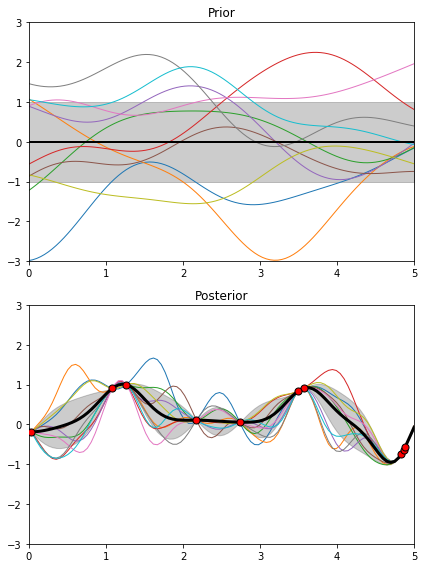
\includegraphics[width=0.6\linewidth]{gp.png}
	\caption{Will add caption later}
	\label{fig:gp}
\end{figure}

When we have more data points coming in, the uncertainty from the posterior distribution will be decreased. Hence, our prediction will become more and more confident when we have more and more data. For traditional parametric methods, the model will tend to overfit the training data when the size of training set grows. However, for Gaussian Processes, since we are not assuming any specific form of the predicted function, we do not have to worry about overfitting. There are still some flexibility left (specified by the variance of the posterior Gaussian distribution), even we have a lot of observation data points added to the  prior distribution. 

\subsubsection{Weight-space View}
EXPAND LATER
\subsubsection{Function-space View}
If we consider a Gaussian Process as a continuous stochastic process, then it defines a probability distribution for functions \cite[Papoulis]{Papoulis}. Since a multivariate Gaussian distribution can be completely specified by its mean and covariance, by definition \ref{def:gp}, then a Gaussian Process can be fully specified by its mean function and covariance function \cite[Rasmussen and Williams]{RandW}. If we define the mean function as $m(\vec{x})$ and covariance function $k(\vec{x},\vec{x'})$ of a real-valued Gaussian Process $f(\vec x)$ as
\begin{equation} \label{}
\begin{split}
m(\vec{x}) & = \EE \left[ f(\vec x)\right] \\
k(\vec{x},\vec{x'}) & = \EE \left[ \left( f(\vec x)-m(\vec{x})\right)\left( f(\vec x')-m(\vec{x'})\right)\right] 
\end{split}
\end{equation}

and then we can write the Gaussian Process $f(\vec x)$ as
\begin{equation} \label{}
f(\vec x) \  \sim \ \GP\left(m(\vec{x}),k(\vec{x},\vec{x'})  \right).
\end{equation}

Suppose we choose a finite subset of random variables $\vec f$ from the Gaussian Process $f(\vec x)$, with the corresponding index set $\mathcal X$, then by definition of Gaussian Process, we know the distribution of $\vec f$:
\begin{equation} \label{}
p\left(\vec f \mid \mathcal X\right)\ =\ \mathcal N \left(\vec m , K \right),
\end{equation}
where $\mathcal N \left(\vec m , K \right)$ denotes a multivariate Gaussian distribution with mean $\vec m$ and covariance $K$. 
In our task, the index set $\mathcal X$ can be a subset of $\mathbb R ^d$, where $d$ is the dimension of our input space. Usually we take the mean function to be a constant function equals to zero for notational simplicity. In practice, one can subtract the mean to achieve this. 

If we estimate our target function $f(\vec x)$ as a Gaussian process, then we need to check if the $consistency$ requirement of estimator is fulfilled. We can easily do this by the marginalization property of multivariate Gaussian distributions. The marginalization property tells us that if 
\begin{equation*} \label{}
\left(\vec f_1, \vec f_2\right)\ \sim \ \mathcal N \left(\vec m , K \right),
\end{equation*}

then we also have 
\begin{equation*} \label{}
\begin{split}
\vec f_1\ & \sim \ \mathcal N \left(\vec m_1 , K_{11} \right)\\
\vec f_2\ & \sim \ \mathcal N \left(\vec m_2 , K_{22} \right).
\end{split}
\end{equation*}
where $K_{11}$ and  $K_{22}$ are sub-matrices of $K$. We prove this relationship in the following:
\begin{proof}
	We prove the marginal density $p(\vec f_1)$ follows Gaussian distribution. First, by definition of marginalization, we have
	\begin{equation*} \label{}
	p(\vec f_1) = \int p(\vec f_1,\vec f_2)d \vec f_2,
	\end{equation*}
	where 
	\begin{equation*} \label{}
	p(\vec f_1,\vec f_2) = \frac{1}{(2\pi)^{n/2}\sqrt{\det K}}\exp{(E)}
	\end{equation*}
	and $E$ is given by
		\begin{equation*} \label{}
		\begin{split}
		E &= -\frac{1}{2}\left(\vec f_2-(\vec m_2 - \vec\Lambda_{22}^{-1} \vec\Lambda_{21}(\vec f_1 - \vec m_1))\right)^T\vec\Lambda_{22}\left(\vec f_2-(\vec m_2 - \vec\Lambda_{22}^{-1} \vec\Lambda_{21}(\vec f_1 - \vec m_1))\right)\\
		&+\frac{1}{2}\left(\vec f_1^T \vec\Lambda_{12}\Lambda_{22}^{-1}\Lambda_{21}\vec f_1 - 2\vec f_1^T \vec\Lambda_{12}\Lambda_{22}^{-1}\Lambda_{21}\vec m_1 + \vec m_1^T \vec\Lambda_{12}\Lambda_{22}^{-1}\Lambda_{21}\vec m_1\right)\\
		&-\frac{1}{2}\left(\vec f_1^T\Lambda_{11}\vec f_1 - 2\vec f_1^T\Lambda_{11}\vec m_1 + \vec m_1^T\Lambda_{11}\vec m_1\right)\\
		&=-\frac{1}{2}\left(\vec f_2-(\vec m_2 - \vec\Lambda_{22}^{-1} \vec\Lambda_{21}(\vec f_1 - \vec m_1))\right)^T\vec\Lambda_{22}\left(\vec f_2-(\vec m_2 - \vec\Lambda_{22}^{-1} \vec\Lambda_{21}(\vec f_1 - \vec m_1))\right)\\
		&-\frac{1}{2}\left(\vec f_1 - \vec m_1\right)^T\left(\vec\Lambda_{11}-\vec\Lambda_{12}\vec\Lambda_{22}^{-1}\vec\Lambda_{21}\right)\left(\vec f_1 - \vec m _1 \right)
		\end{split}
		\end{equation*}
	where $\vec\Lambda$ is the information matrix and
	\begin{equation*} \label{}
	\vec \Lambda = K^{-1} = 
	\begin{pmatrix}
	\vec\Lambda_{11} & \vec\Lambda_{12}\\
	\vec\Lambda_{21} & \vec\Lambda_{22}
	\end{pmatrix}.
	\end{equation*}
	Using the \textit{matrix inversion lemma} (see Appendix), we have
	\begin{equation*} \label{}
	K_{11}^{-1} = \vec\Lambda_{11}-\vec\Lambda_{12}\vec\Lambda_{22}^{-1}\vec\Lambda_{21},
	\end{equation*}
	combined with the line above, we get
	\begin{equation*} \label{}
	p(\vec f_1,\vec f_2) = \frac{1}{(2\pi)^{n/2}\sqrt{\det K}}\exp{(E_1)}\exp{(E_2)},
	\end{equation*}
	where
	\begin{equation*} \label{}
	\begin{split}
	E_1 &=-\frac{1}{2}\left(\vec f_2-(\vec m_2 - \vec\Lambda_{22}^{-1} \vec\Lambda_{21}(\vec f_1 - \vec m_1))\right)^T\vec\Lambda_{22}\left(\vec f_2-(\vec m_2 - \vec\Lambda_{22}^{-1} \vec\Lambda_{21}(\vec f_1 - \vec m_1))\right)\\
	E_2 & = -\frac{1}{2}\left(\vec f_1 - \vec m_1\right)^T\left(\vec\Lambda_{11}-\vec\Lambda_{12}\vec\Lambda_{22}^{-1}\vec\Lambda_{21}\right)\left(\vec f_1 - \vec m _1 \right).
	\end{split}
	\end{equation*}
	Since $E_2$ is independent of $\vec f_1$, we have
	\begin{equation*} \label{}
	p(\vec f_1) = \frac{1}{(2\pi)^{n/2}\sqrt{\det K}}\int \exp{(E_1)}d\vec f_2\exp{(E_2)}.
	\end{equation*}
	Integral of a probability density function is one, we get
	\begin{equation*} \label{}
	\int \exp{(E_1)}d\vec f_2 = (2\pi)^{n_2/2}\sqrt{\det \vec \Lambda_{22}^{-1}}
	\end{equation*}
	plug this into the line above, we get
	\begin{equation*} \label{}
	p(\vec f_1) = \frac{\sqrt{\det \vec \Lambda_{22}^{-1}}}{(2\pi)^{n_1/2}\sqrt{\det K}} \exp{\left(-\frac{1}{2}\left(\vec f_1 - \vec m_1\right)^TK_{11}^{-1}\left(\vec f_1 - \vec m _1 \right)\right)}.
	\end{equation*}
	Again, by the \textit{matrix inversion lemma}, we have
	\begin{equation*} \label{}
	\begin{split}
	\det K&= \det K_{11}\det(K_{22}-K_{21}K_{11}^{-1}K_{12})\\
	\vec \Lambda_{22}^{-1} &= K_{22}-K_{21}K_{11}^{-1}K_{12}.
	\end{split}
	\end{equation*}
	Plug those results into the previous line, we get
	\begin{equation*} \label{}
	p(\vec f_1) = \frac{1}{(2\pi)^{n_1/2}\sqrt{\det K_{11}}} \exp{\left(-\frac{1}{2}\left(\vec f_1 - \vec m_1\right)^TK_{11}^{-1}\left(\vec f_1 - \vec m _1 \right)\right)}.
	\end{equation*}
	which proves that $\vec f_1\sim\mathcal{N}(\vec m_1,K_{11})$.
\end{proof}
Now that we have the $consistency$ requirement fulfilled, we can introduce Gaussian Process Regression models.
\subsection{Gaussian Process Regression}
So far, we have introduced Gaussian Processes. In order to solve the regression problem, we first define a prior distribution of our target functions by a Gaussian process, then apply Bayesian inference to get the posterior distribution of our predictions. 

We start by modelling our target latent function $\vec f$ by a zero mean Gaussian Process, then $\vec f$ has prior distribution:
\begin{equation} \label{noise-free}
	\vec f \sim \mathcal{N}(\vec 0, K),
\end{equation}
where $K$ is the covariance matrix.

First, we assume the special case where our target functions are noise-free. Suppose we have observed data $\{(\vec x_i,f_i)|i=1,...,n\}$, we want to infer the value of our target function at input points $\{\vec x_j | j = 1,...,n_*\}$. We call $\vec f$ as training outputs and $\vec f_*$ as test outputs. From the prior distribution, we know 
$\vec f$ and $\vec f_*$ have joint distribution
\begin{equation} \label{}
	\begin{bmatrix}
	\vec f\\
	\vec f_*
	\end{bmatrix}
	\sim
	\mathcal{N}\left(\vec 0, 
	\begin{bmatrix}
	K(X,X) & K(X,X_*)\\
	K(X_*,X) & K(X_*,X_*)
	\end{bmatrix}
	\right).
\end{equation}
$K(X,X)$ denotes the covariance matrix of $n$ training data points, $K(X_*,X_*)$ denotes the covariance of $n_*$ test data points and $K(X_*,X)$ denotes the cross-covariance of training and test data points. To get the distribution of our prediction on the test data set, we just condition the joint Gaussian prior distribution on the training data set. Then we get
\begin{equation} \label{eq:pred1}
	\vec f_* | X_*, X, \vec f \sim \mathcal N (\vec m_*, \vec V_*),
\end{equation}
where
\begin{equation} \label{eq:pred2}
\begin{split}
\vec m_* &= K(X_*,X)K(X,X)^{-1}\vec f,\\
\vec V_* &= K(X_*,X_*) - K(X_*,X)K(X,X)^{-1}K(X,X_*).
\end{split}
\end{equation}

ADD PROOF FOR THE ABOVE RESULT.

Our prediction of the test set is a posterior gaussian distribution with mean $\vec m_*$ and covariance $\vec V_*$.  Notice that in our prediction, rather than giving specific parametric relationship between the test input $\vec X_*$ and the prediction value, we just give a Gaussian distribution inferred from our prior distribution and observation. If we want to get an exact value of $\vec f_*$ for prediction, we can sample from the posterior distribution or simply take the mean $\vec m_*$ as our prediction. For more on this, see section \ref{sec:decision_theory}. We can also get the variance $v_*$ of each individual element in vector  $\vec f_*$ from the covariance matrix $\vec V_*$. The smaller the variance is, the more confident we are about the prediction. 

In most real-life application, it is more realistic to incorporate noise in our target values. We can denote the noisy target values as $\vec y$ in training set. We then write the noisy value as $\vec y = f(\vec x) + \vec\epsilon$. Assuming identical, independent Gaussian noise $\vec \epsilon$ with mean $0$ and variance $\sigma^2_n$, then the covariance on the noisy observation is
\begin{equation*} \label{}
\mathrm{cov} (y_i,y_j) = k(\vec x_i,\vec x_j) + \sigma^2_n \delta_{ij}
\end{equation*}
where $\delta_{ij}$ is a Kronecker delta which is $1$ is $i=j$ and $0$ otherwise. The above relationship is vector form is
\begin{equation} \label{cov_y}
\mathrm{cov} (\vec y) = K(X,X) + \sigma^2_n \vec I,
\end{equation}
where the identity matrix $\vec I$ comes from the independence assumption of the noise. Then we can write the joint prior distribution of noisy training data and test data as
\begin{equation} \label{}
	\begin{bmatrix}
	\vec y\\
	\vec f_*
	\end{bmatrix}
	\sim
	\mathcal{N}\left(\vec 0, 
	\begin{bmatrix}
	K(X,X)+ \sigma^2_n \vec I & K(X,X_*)\\
	K(X_*,X) & K(X_*,X_*)
	\end{bmatrix}
	\right).
\end{equation}
Then by the same derivation to eq. \ref{eq:pred1} and \ref{eq:pred2}, we get the prediction for test data. The posterior distribution is 
\begin{equation} \label{eq:pred3}
	\vec f_* | X_*, X, \vec y \sim \mathcal N (\widehat{\vec m_*}, \widehat{\vec V_*}),
\end{equation}
where
\begin{equation} \label{eq:pred4}
\begin{split}
\widehat{\vec m_* }&= K(X_*,X)[K(X,X)+ \sigma^2_n \vec I]^{-1}\vec y,\\
\widehat{\vec V_*} &= K(X_*,X_*) - K(X_*,X)[K(X,X)+ \sigma^2_n \vec I]^{-1}K(X,X_*).
\end{split}
\end{equation}

Notice that though we assume the mean function as constantly zero in the prior distribution, we get non-zero mean function in the posterior distribution for the test data set. This can be interpreted as after observing the training set, we have more information about the distribution of the test set. Also, different from a parametric model, when trained, the model can basically throw away all the training data, the Gaussian Process Regression model needs to store all the training data for prediction. For a parametric model, the goal is to find the predefined parametric relationship between features and targets, once done that, we don't need the training data for prediction. The features, ${\vec x^*_i | i=1,...,n^*}$, will give all the information we need for prediction $\vec y^*_i$'s. However, in Gaussian Process Regression model, the prediction eq. \ref{eq:pred3} and eq. \ref{eq:pred4} need the information from training set to get the posterior distribution of the test set.

\subsection{Predicition from Gaussian Process Regression}\label{sec:decision_theory}
Form eq. \ref{eq:pred3}, we know that the posterior distribution of test data is Gaussian with mean and variance given in eq.\ref{eq:pred4}. But if we want an explicit prediction for our target function rather than a distribution, what is the value then? One intuitive answer would be the mean of posterior distribution. In practice, this prediction is appropriate in most real-life tasks. There are in-depth explanation in \cite[Rasmussen and Williams, sec 2.4]{RandW}, we give a summary of the rationale in the following.

To find a optimal prediction value, we need a way to measure our performance. Let's define a \textit{loss function}, $\mathcal{L}(\hat y,y)$, which specifies the loss between the prediction, $\hat y$ and the true value, $y$. The loss function can be \textit{mean squared error} or \textit{mean absolute error} which are both symmetric loss functions.

We want to give a prediction value that produces the minimum loss possible. But how do we achieve that when we don't know the true value? According to \cite[Rasmussen and Williams, sec 2.4]{RandW}, we can minimize the expected loss, by averaging the loss with respect to the posterior distribution, which is 
\begin{equation}\label{loss1}
\tilde{R}_{\mathcal{L}}(\hat y|\vec x_*)\ = \ \int\mathcal{L}(y_*,\hat y)p(y_*|\vec x_*)dy_*.
\end{equation}\label{loss2}
Our best prediction is the one that minimizes this loss, i.e.
\begin{equation}
y_{optimal}|\vec x_*\ = \ \underset{\hat y}{\mathrm{argmin}}\tilde{R}_{\mathcal{L}}(\hat y|\vec x_*).
\end{equation}
For \textit{mean squared error} loss function, the minimum occurs at the mean of $y_*$. For \textit{mean absolute error} loss function, the minimum occurs at the median of $y_*$. In our case, the distribution of $y_*$ is Gaussian, so the mean and median coincide. Furthermore, for other symmetric loss function and symmetric posterior distribution, the optimal prediction occurs at the mean of the distribution. For asymmetric loss functions, the optimal prediction can be computed from eq. \ref{loss1} and eq. \ref{loss2}. For more detail, see \cite[Berger]{Berger}.

\newpage
\section{Model Selection}
When modelling our target function as a zero mean Gaussian process regression(GPR), i.e.
\begin{equation*} \label{}
f(\vec x) \  \sim \ \GP\left(\vec 0,k(\vec{x},\vec{x'})  \right).
\end{equation*}
the main task will be to find a good configuration of covariance matrix, generated by kernel function $k$ and a set of $hyperparameters$ that gives the best performance. The model selection is a combination of choosing a good kernel function and optimizing $hyperparameters$ of the kernel function. In this section, we will discuss several aspects of model selection, namely covariance matrix, kernel functions, $hyperparameters$ optimization.

\subsection{Marginal Likelihood of the training data}\label{lik}
From eq. \ref{noise-free}, we know that the noise-free prior follow multivariate Gaussian distribution with mean $\vec 0$ and covariance $K(X,X)$. By Bayes' theorrm, the marginal likelihood of our noisy training data is the intergral of the likelihood times prior, whcih is 

\begin{equation}
     p(\vec y|X)\, = \, \int p(\vec y|\vec f, X)p(\vec f|X)d\vec f.
\end{equation}

The term \textit{marginal} likelihood means the marginalization over the function values $\vec f$. If we assume i.i.d. Gaussian noise, then we have $\vec y = f(\vec x) + \vec\epsilon$, where $\vec\epsilon \sim \mathcal{N}(\vec 0, \sigma^2_n)$. Let $K_y = K + \sigma^2_nI$, then by eq. \ref{cov_y}. we have
\begin{equation}
\vec y \  \sim \ \mathcal N \left(\vec 0,K_y  \right).
\end{equation}
Since the likelihood of a Gaussian distribution involves exponential term, we take the logarithm of it. So the log likelihood of $\vec y$ given $\vec X$ and $\vec \theta$ is
\begin{equation}\label{log-likelihood}
\log p(\vec y|\vec X, \vec \theta)=-\frac{1}{2}\vec y^T K_y^{-1}\vec y-\frac{1}{2}\log|K_y| - \frac{n}{2}\log 2\pi,
\end{equation}
where $\vec \theta$ is parameters in kernel function $k$.

\subsection{Kernel functions}
A kernel function (also called a covariance function), $k$ governs the behaviour and property of a zero-mean Gaussian process. Since for any element, $K_{ij}$ in the covariance matrix $K$, we know $K_{ij} = k(\vec x_i,\vec x_j)$. Then the relationship of covariance matrix $K$ and kernel function $k$ is
\begin{equation}\label{cov_mat}
K = 
\begin{bmatrix}
k(\vec x_1,\vec x_1) & k(\vec x_1,\vec x_2)& \dots& k(\vec x_1,\vec x_n)\\
k(\vec x_2,\vec x_1) & k(\vec x_2,\vec x_2)& \dots& k(\vec x_2,\vec x_n)\\
\vdots & \vdots  & \ddots & \vdots \\
k(\vec x_n,\vec x_1) & k(\vec x_n,\vec x_2)& \dots& k(\vec x_n,\vec x_n)
\end{bmatrix}
\end{equation}

\begin{figure}[h!]
	\centering
	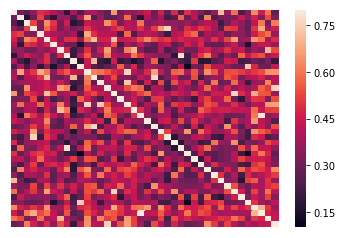
\includegraphics[width=0.4\linewidth]{cov1.png}
	\vspace{2em}
	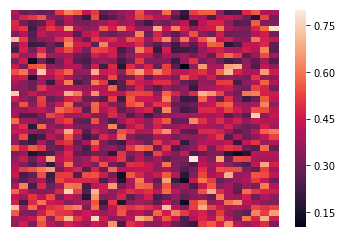
\includegraphics[width=0.4\linewidth]{cov2.png}}
	\caption{Covariance matrix}
\end{figure}

A kernel function in some sense measures the similarity between two data points in the input space. The basic assumption in GPR is that two points are close in the input space should be more likely to have a similar target value. 

Since a covariance matrix is always positive-semidefinite\footnotemark[1] and symmetric, for a function to be qualified as a kernel function, it must be positive-semidefinite\footnotemark[2] and symmetric in the sense that $k(\vec x_i,\vec x_j) = k(\vec x_j,\vec x_i)$\cite[Rasmussen and Williams, sec 4.1]{RandW}.

\footnotetext[1]{
	A symmetric $n\times n$ real matrix $\vec M$ is said to be positive-semidefinite(PSD) if $\vec v^T\vec M\vec v$ is non-negative for all $\vec v$ in $\RR^n$.
	}
\footnotetext[2]{
	A $kernel$ is said to be positive-semidefinite if 
	\[
		\int k(\vec x,\vec x')f(\vec x)f(\vec x')d\mu(\vec x)d\mu(\vec x')\, \geq 0,
	\]
	for all $f\in L_2(\mathcal X,\mu)$, $\mathcal X$ is the input space and $\mu$ is a measure.
	}

\subsubsection{Several Common Kernel functions}
Kernel function map $\vec x,\vec x' \in \mathcal X$ into $\RR$. We measure the similarity of $\vec x,\vec x'$ in $\mathcal X$ by the result from the kernel function.

A stationary kernel function is a function whose value only depends on the difference between $\vec x$ and $\vec x'$. We write $k$ to take only single argument $\vec r = \vec x - \vec x'$. 
\subsubsection*{Squared Exponential Kernel Functions}
The mostly commonly used stationary kernel function is the \textit{squared exponential}(SE) kernel function, which has the form
\begin{equation}\label{SE_kernel}
k_{SE}\, = \, \sigma^2\exp\left(-\frac{\vec r^2}{2l^2}\right),
\end{equation}
the parameter $l$ is the \textit{characteristic length-scale} and $\sigma$ controls the magnitude of function value. The \textit{squared exponential} kernel function is also known as the \textit{radial basis function}. This kernel function has derivatives at all orders, which means Gaussian process with this kernel will be very smooth. For detailed explanation, please see \cite[Rasmussen and Williams, sec 4.2]{RandW}. Sometimes, it is not very ideal to assume such strong smoothness for functions in real applications, so we introduce another family of stationary kernel functions, namely the \textit{Mat\'ern class}\cite[Stein]{Stein}.

\subsubsection*{Mat\'ern Class of Kernel Functions}
This class of kernel functions was named after the work of Mat\'ern. The general form of \textit{Matern class} kernel functions is given by
\begin{equation}
k_{Matern}(\vec r) = \frac{2^{1-\nu}}{\Gamma{(\nu)}}\left(\frac{\sqrt{2\nu}\vec r}{l}\right)^\nu K_\nu \left(\frac{\sqrt{2\nu}\vec r}{l}\right),
\end{equation}
where $\nu$ and $l$ are positive parameters and $K_\nu$ is a second kind modified Bessel function\cite[Abramowitz and Stegun]{Ab_St}. When $\nu \rightarrow \infty$, we obtain the SE kernel function. For smaller $\nu$, the resulting Gaussian process has a rougher path than those from a SE kernel. The most commonly exploited cases in machine learning is when $\nu = 3/2$ and $ 5/2$\cite[Rasmussen and Williams, sec 4.2]{RandW}. These two kernel functions are of the forms
\begin{equation}
\begin{split}
k_{\nu = 3/2}(\vec r) &=\left(1+\frac{\sqrt{3}\vec r}{l}\right)\exp\left(-\frac{\sqrt{3}\vec r}{l}\right),\\
k_{\nu = 5/2}(\vec r) &=\left(1+\frac{\sqrt{5}\vec r}{l}+\frac{5\vec r^2}{3l^2}\right)\exp\left(-\frac{\sqrt{5}\vec r}{l}\right).
\end{split}
\end{equation}
For $\nu\geq 7/2$, the resulting Gaussian process will become very smooth\cite[Rasmussen and Williams, sec 4.2]{RandW}.

ADD GRAPH TO ILLUSTRATE DIFFERENCE IN "SMOOTHNESS" BETWEEN DIFFERENT KERNELS

Stationary kernels will give the same value as long as the difference between $\vec x$ and $\vec x'$ is the same. Hence, stationary kernels are translation invariant. When we want to incorporate effects of translation in feature space, we need to introduce non-stationary kernel functions.

\begin{table}[h!]
	\begin{center}
		\caption{Training data metrics}
		\label{tab:table1}
		\begin{tabular}{c|c|c|c}
			\mbox{Difference} & \mbox{RBF} & \mbox{Matern32}& \mbox{Matern52}\\ %\mbox{RBF + Linear}& \mbox{Matern32 + Linear}& \mbox{Matern52 + Linear}\\
			\hline
			10&47.94&58.51&56.10\\
			100&74.13&	83.42&	81.23\\
			1000&94.06&	98.35&	97.52\\
			10000&99.96&	99.98&	99.98
		\end{tabular}
	\end{center}
\end{table}

\begin{table}[h!]
	\begin{center}
		\caption{Testing data metrics}
		\label{tab:table1}
		\begin{tabular}{c|c|c|c}
			\mbox{Difference} & \mbox{RBF} & \mbox{Matern32}& \mbox{Matern52}\\ %\mbox{RBF + Linear}& \mbox{Matern32 + Linear}& \mbox{Matern52 + Linear}\\
			\hline
			10&27.45&	30.76&	29.56\\
			100&41.58&	44.59&	45.29\\
			1000&65.83&	68.34&	68.44\\
			10000&88.38&	88.08&	87.88
		\end{tabular}
	\end{center}
\end{table}

\subsubsection*{Linear Kernel Functions}
A linear kernel function has the form
\begin{equation}
k_{Linear} = \frac{\vec x \cdot \vec x'}{l},
\end{equation}
where $l$ is the \textit{characteristic length-scale}.

\subsubsection*{Combining Kernel Functions}
For most real-life tasks, using vanilla kernel functions described above may not generate ideal result. We can construct new kernel functions from these vanilla kernel functions by addition, multiplication, convolution and other methods. Adding two kernel functions is equivalently modelling the resulting Gaussian process by the sum of two independent Gaussian processes\cite[Rasmussen and Williams, sec 4.2]{RandW}.

\begin{table}[h!]
	\begin{center}
		\caption{Training data metrics}
		\label{tab:table1}
		\begin{tabular}{c|c|c|c}
			\mbox{Difference} &\mbox{RBF+Linear}& \mbox{Matern32+Linear}& \mbox{Matern52+Linear}\\
			\hline
			10&31.30&	45.19&	18.25\\
			100&56.18&	75.07&	34.17\\
			1000&85.61&	96.25&	63.11\\
			10000&99.63	&100.00	&90.27
		\end{tabular}
	\end{center}
\end{table}

\begin{table}[h!]
	\begin{center}
		\caption{Testing data metrics}
		\label{tab:table1}
		\begin{tabular}{c|c|c|c}
			\mbox{Difference} &\mbox{RBF+Linear}& \mbox{Matern32+Linear}& \mbox{Matern52+Linear}\\
			\hline
			10&23.75&	28.36&	15.83\\
			100&39.48&	41.98&	31.16\\
			1000&65.23&	68.74&	56.81\\
			10000&89.78&	90.28&	85.27
		\end{tabular}
	\end{center}
\end{table}


\subsubsection{Optimizing Kernel Parameters}
Each kernel function has a set of parameters which determines properties of the kernel function. In Gaussian process regression, since these parameters specify distributions of the parameters of target function, so we call them $hyperparameters$ of the model. In the training process of our model, we want to find a optimal set of $hyperparameters$ in the sense that the log likelihood of our training data define in eq. \ref{log-likelihood} is maximised. We will discuss in detail about training methods in the following subsection.

\subsection{Training Methods}
In this subsection, we will suppose several objective functions for training and use gradient decent based algorithm for optimisation.

\subsubsection{Maximum Likelihood}
Recall from eq. \ref{log-likelihood}, we define the marginal likelihood of training data
\begin{equation}
\log p(\vec y|\vec X, \vec \theta)=-\frac{1}{2}\vec y^T K_y^{-1}\vec y-\frac{1}{2}\log|K_y| - \frac{n}{2}\log 2\pi,
\end{equation}
where $K_y = K_{\vec f}+\sigma^2 I$ is the covariance matrix for the noisy targets value $\vec y$. $K_f$ is the covariance matrix of latent function $\vec f$ and $\sigma^2$ is the variane of i.i.d. Gaussian noise. We can interpret the first term in the marginal likelihood $-\frac{1}{2}\vec y^T K_y^{-1}\vec y$ as the data-fit since it is the only term involves target values. The second term $-\frac{1}{2}\log|K_y|$ is the complexity penalty since it only depends on the covariance matrix. The third term $- \frac{n}{2}\log 2\pi$ is the normalization constant\cite[Rasmussen and Williams, sec 5.4]{RandW}. As \textit{length-scale} increases, $K_y^{-1}$ decreases and $\log|K_y|$ increases. So we want to find a set $\vec \theta$ such that

\begin{equation}
    \vec{\hat \theta} = \ \underset{\vec \theta \in \vec \Theta}{\mathrm{argmax}}\log p(\vec y|\vec X, \vec \theta).
\end{equation}

In practice, in order to find $\vec{\hat \theta}$ that maximises the log marginal likelihood, we first take partial derivatives of the the log marginal likelihood with respect to each element of the hyperparameter vector $\vec \theta$. Here, we use vector $\vec \theta$ to denote all the hyperparameters in our chosen kernel function.  Let $\vec \theta_i$ be $i^{th}$ element in $\vec \theta$, then the partial derivative of log marginal likelihood w.r.t. $\vec \theta_i$ is 
\begin{equation}
\begin{split}
\frac{\partial}{\partial \vec \theta_i}\log p(\vec y|\vec X, \vec \theta) & = -\frac{1}{2}\vec y^T \frac{\partial K^{-1}}{\partial \vec \theta_i}\vec y-\frac{1}{2}\frac{\partial \log|K|}{\partial \vec \theta_i}\\
& = -\frac{1}{2}\vec y^T\left(  -K^{-1} \frac{\partial K}{\partial \vec \theta_i} K^{-1} \right)\vec y - \frac{1}{2}\text{tr} \left(K^{-1}\frac{\partial K}{\partial\vec \theta_i}\right)\\
&= \frac{1}{2}\vec y^TK^{-1} \frac{\partial K}{\partial \vec \theta_i} K^{-1} \vec y - \frac{1}{2}\text{tr} \left(K^{-1}\frac{\partial K}{\partial\vec \theta_i}\right)\\
& = \frac{1}{2}\text{tr} \left( (\vec \alpha\alpha^T - K^{-1})\frac{\partial K}{\partial\vec \theta_i}\right) \text{, where } \vec \alpha = K^{-1} \vec y.
\end{split}
\end{equation}
Notice that $\frac{\partial K}{\partial\vec \theta_i}$ denotes the matrix of element-wise derivatives. Then in each iteration, we update our the parameters $\vec\theta^n_i$ by
\begin{equation}
\vec\theta^n_i = \vec\theta^{n-1}_i - \eta\frac{\partial}{\partial \vec \theta_i}\log p(\vec y|\vec X, \vec \theta) 
\end{equation}
where $\eta$ is a predefined learning rate. 

The main computational complexity of computing this partial derivative lies in the computing of $K^{-1}$, which is of order $\mathcal O(n^3)$ for a $n$ dimensional matrix $K$. After we have computed partial derivatives for every hyperparameters, we update each of them using a gradient decent based optimizer. Many well known packages in major programming languages have those optimizer built-in. We use Python for our implementation. One can find several more efficient optimizers such as RMSPropOptimizer and AdamOptimizer in Python. In practice, we will set our objective function to be the negative log likelihood, then we use optimizer to minimise our objective function w.r.t. hyperparameters. For those optimizers mentioned above, We can also use adaptive learning rate during optimising operation for better performance when approaching to the minimal point. By adaptive learning rate, we mean learning rate decays by a certain method. For instance, the time-based decay is specified by $\eta = \eta_0/(1+k*t)$, where $\eta_0$ is the initial learning rate, $k$ is a hyperpamater that governs the decay speed and $t$ is the iterations that have passed\cite[Bengio]{Bengio}.

\subsubsection{LOO-CV Based Objective Functions}
We can also define our objective function as the leave-one-out cross validation (LOO-CV) based predictive measure. Cross Validation (CV) baed predictive measure has been successfully used in many model selection tasks in machine learning\cite[Cawley and Talbot]{Cawley_Talbot}\cite[Sundararajan and Keerthi]{Sundararajan_Keerthi}. 

Predictive Sample Reuse(PSR) methods was introduced by Geisser\cite{Geisser} to be applied for both model selection and parameters optimisation problem. The basic idea is to define a partition of training data $P(N,n,\Gamma)$ such that such that $P_{N-n}^i$ is the predictive probability of $i^{th}$ subset of size $n$ in the partition. Leave-one-out cross validation is the special case when we take the size of element in the partition to be $n=1$.

The predictive log likelihood when leaving out training case $i$ is
\begin{equation}\label{GPP_1}
\log p(y_i|\vec X,\vec y_{-i},\vec \theta) = -\frac{1}{2}\log\sigma^2_i - \frac{(y_i - \mu_i)^2}{2\sigma^2_i} - \frac{1}{2} \log 2 \pi, 
\end{equation}
where $\vec y_{-i}$  means all targets value except the $i^{th}$ value, $\mu_i$ and $\sigma_i$ are calculated according to eq. \ref{eq:pred4}. The training data are taken to be $(\vec X_{-i},\vec y_{-i})$. We take our objective function to be the average negative predictive log likelihood, which is given by
\begin{equation}\label{GPP}
\begin{split}
G(\vec X,\vec y, \vec \theta) &= -\frac{1}{n}\sum_{i=1}^{n}\log p(y_i|\vec X,\vec y_{-i},\vec \theta)\\
\end{split}
\end{equation}
This objective function is known as Geisser's surrogate Predictive Probability(GPP), first supposed by Geisser and Eddy in \cite{Geisser_Eddy}. It is also called \textit{pseudo}-likelihood by Rasmussen and Williams in \cite[sec. 5.4]{RandW}. 

The main computational cost in calculating GPP is in the calculation of the predictive mean $\mu_i$ and predictive variance $\sigma^2_i$, which are dominated by the inversion of the matrix $K$ in eq. \ref{eq:pred4}. The expression for $\mu_i$ and $\sigma^2_i$ was calculated in \cite{Sundararajan_Keerthi}, and they are
\begin{equation}\label{GPP_2}
\begin{split}
\mu_i &= y_i - [K^{-1}\vec y]_i/[K^{-1}]_{ii},\\
\sigma^2_i &= 1/[K^{-1}]_{ii}.
\end{split}
\end{equation}

Plug in these expressions into eq. \ref{GPP_1} and eq. \ref{GPP} to get the objective function. The next step is to calculate the partial derivatives of the objective function with respect to hyperparameters. We first use the expression in eq. \ref{GPP_2} to calculate the partial derivatives of the predictive mean and variance
\begin{equation}\label{GPP_3}
\begin{split}
\frac{\partial\mu_i}{\partial \vec \theta_j} &= \frac{[Z_j \vec \alpha]_i}{[K^{-1}]_{ii}} - \frac{\vec \alpha_i[Z_j K^{-1}]_{ii}}{[K^{-1}]^2_{ii}},\\
\frac{\partial\sigma^2_i}{\partial \vec \theta_j} &= \frac{[Z_j K^{-1}]_{ii}}{[K^{-1}]^2_{ii}},
\end{split}
\end{equation}
where $\vec \alpha = K^{-1}\vec y$ and $Z_j = K^{-1}\frac{\partial K}{\partial \vec \theta_j}$. Using chain rule and eq. \ref{GPP_1} to calculate the partial derivatives of eq.\ref{GPP}
\begin{equation}\label{GPP_derivative}
\begin{split}
\frac{\partial G(\vec X,\vec y, \vec \theta)}{\partial \vec \theta_j} &= -\frac{1}{n}\sum_{i=1}^{n}\frac{\partial \log p(y_i|\vec X,\vec y_{-i},\vec \theta)}{\partial \mu_i}\frac{\partial \mu_i}{\partial \vec \theta_j} + \frac{\partial \log p(y_i|\vec X,\vec y_{-i},\vec \theta)}{\partial \sigma^2_i}\frac{\partial \sigma^2_i}{\partial \vec \theta_j}\\
&=-\frac{1}{n}\sum_{i=1}^{n}\left(\alpha_i[Z_j \vec{\alpha}]_i - \frac{1}{2}\left(1+\frac{\alpha^2_i}{[K^{-1}]_{ii}}\right)[Z_j K^{-1}]_{ii}\right)/[K^{-1}]_{ii}.
\end{split}
\end{equation}
With partial derivatives calculated, we can use gradient decent based optimizer to minimise our objective function $G(\vec X,\vec y, \vec \theta)$.

Another LOO-CV based objective function is Geisser's Predictive mean square Error(GPE)\cite[Geisser and Eddy]{Geisser_Eddy}\cite[Sundararajan and Keerthi]{Sundararajan_Keerthi}. GPE is define by $\frac{1}{n}\sum_{i=1}^{n}\mathbb E[(y_i-\hat{y}_i)^2]$, where $\hat{y}_i$ is the predicted value from the model using data set $(\vec X_{-i}.\vec y_{-i})$ and $y_i$ is the true target value.The objective function corresponding to GPE is
\begin{equation}\label{GPE}
\begin{split}
G_E(\vec X,\vec y, \vec \theta) = \frac{1}{n}\sum_{i=1}^{n}\int (y_i-\hat{y}_i)^2 p(\hat y_i|\vec X,\vec y_{-i},\vec \theta)d\hat y_i,
\end{split}
\end{equation}
where $\hat y_i$ follows a Gaussian distribution with mean $\mu_i$ and variance $\sigma^2_i$ given by eq. \ref{GPP_2}. Thanks to the analytical tractability of Gaussian distribution, we can simplify the objective function as 
\begin{equation}\label{GPE_1}
G_E(\vec X,\vec y, \vec \theta) = \frac{1}{n}\sum_{i=1}^{n}(y_i-\mu_i)^2+\sigma^2_i.
\end{equation}
We can see from the expression of $G_E$, this objective function will aim to minimise the deviation between the predictive mean and the true value as well as the predictive variance. We can also use chain rule and eq. \ref{GPP_1} to calculate the partial derivatives of GPE objective function
\begin{equation}\label{GPE_derivative}
\frac{\partial G_E(\vec X,\vec y, \vec \theta)}{\partial \vec \theta_j} = \frac{1}{n}\sum_{i=1}^{n}\frac{\partial (y_i-\mu_i)^2}{\partial \mu_i}\frac{\partial \mu_i}{\partial \theta_j}+2\sigma_i\frac{\partial \sigma_i}{\partial \theta_j}.
\end{equation}
Plug in eq. \ref{GPP_3} to get
\begin{equation}\label{GPE_derivative_2}
\frac{\partial G_E(\vec X,\vec y, \vec \theta)}{\partial \vec \theta_j} = \frac{1}{n}\sum_{i=1}^{n}\left([Z_j K^{-1}]_{ii}\left(1+2\frac{\vec\alpha^2_i}{[K^{-1}]_{ii}}\right)-2\vec \alpha_i[Z_j\vec\alpha]_i\right)/[K^{-1}]_{ii},
\end{equation}
where $\vec \alpha = K^{-1}\vec y$ and $Z_j = K^{-1}\frac{\partial K}{\partial \vec \theta_j}$.

Once we have calculated the partial derivatives, we just follow the similar steps in the maximum likelihood case to update the hyperparameters.

The three objective proposed above have similar computational expense, all dominated by the inversion of covariance matrix $K$, which is $\mathcal O(n^3)$. The main difference is that maximum likelihood gives us the probability of training data given the assumption of model while the two LOO-CV based methods estimate the predictive probability and error which gives us a measure of how good is our assumption. 

\subsubsection{Automatic Relevance Determination}
In the previous discussion, we used single scalar value for the \textit{characteristic length-scale} $l$ in hyperparameter $\vec \theta$ for kernels functions. In practice, for multi-dimensional feature space, a universal \textit{characteristic length-scale} for all dimensions may not perform well. Instead, We can assign a \textit{characteristic length-scale} for each dimension. For instance, a SE kernel function in this form is
\begin{equation}\label{SE_ARD}
k_{SE\_ARD}\, = \, \sigma^2\exp\left(-\frac{1}{2}\sum_{i=1}^{d}\frac{\vec r^2_i}{ l^2_i}\right),
\end{equation}
where $\vec r \in \mathbb R^d$, $d$ is the number of dimensions in feature space. ARD stands for automatic relevance determination\cite[Neal]{Neal}. 
From eq.\ref{SE_ARD}, we can see that the inverse of $l_i$ will determine how sensitive the covariance is to the change in $\vec r_i$. For large value of $l_i$, the inverse is close to zero which will make covariance all-most invariant to the change in $\vec r_i$. This effect will determine the relevance of $i^{th}$ dimension of input to the covariance, hence, the name -- automatic relevance determination(ARD).
\newpage

\section{Data Analysis}

\subsection{Data Description}

\subsection{Dimension Reduction}
Due to the computational expense of calculating the inverse of covariance matrix, which is of order $\mathcal O(n^3)$ for a $n$-dimensional positive semi-definite matrix, it is hard to work with large data set in practice. However, for high dimensional input, we have to train our model with a reasonably large amount of data so that on average each dimension is adequately represented. To tackle this dilemma, we need to reduce the dimension of feature space while retaining the information from the original data. In this subsection, we will present two dimension reduction techniques, namely Principal Component Analysis(PCA) and Autoencoder(AE). 

\subsubsection{Principal Component Analysis}
Principal Component Analysis(PCA) is used extensively in statistics for data presentation and dimension reduction. The main purpose of PCA is to find a new coordinate system in which we can express the original data with less dimensions without significant loss of information. We will briefly explanation how PCA works in the following. For detailed discuss about PCA, please see \cite[Jolliffe]{Jolliffe}.

To perform PCA, we first need to standardize the data by subtracting mean and dividing standard deviation. Then calculate the sample covariance matrix of the input data $\vec Q = \frac{1}{n-1}\vec X\vec X^T$, where each column of $\vec X$ is one data point in original input space, $\mathbb R^d$. Then find the eigenvalues $\lambda_1, \cdots,\lambda_d$ of $\vec Q$ and corresponding orthogonal eigenvectors $\vec u_1,\cdots,\vec u_d$. Then sort the eigenvalues in descending order and corresponding eigenvectors. The eigenvector corresponding to the largest eigenvalue is called first \textit{principal component} and so on. To reduce dimensions, we discard those eigenvectors corresponding to eigenvalues that are smaller than a predefined threshold(small eigenvalues correspond to eigenvectors containing less information about the original data). Now we have chosen $k$($<d$) eigenvectors to form our feature matrix $\vec U$ which is of shape $k\times d$. The dimension reduction is done by multiplying $\vec X$ by $\vec U$ from left,
\begin{equation}
\vec X' = \vec U \cdot \vec X
\end{equation}
where $\vec X'$ is a $k\times n$ matrix with each column a transformed data point in reduced input space $\mathbb R^k$.

\subsubsection{Autoencoder}
An autoencoder is a type of feed forward neural network that is mainly used for efficient data encoding\cite[chapter 14]{Deep_Learning}. The most simple case of autoencoder contains three layers, namely input layer, hidden layer and output layer. This type of autoencoder can be divided into two parts: an encoder function and a decoder function. An encoder function takes the original data as input and transform it to a transformed space. Denote the encoder as $\vec h = f(\vec x)$, where $\vec x\in \mathbb R^d, \vec h\in \mathbb R^m$. A decoder function takes $\vec h$ as input and outputs a reconstruction of the original data $\vec x' = g(\vec h)$. We train the model by minimize the reconstruction error between $\vec x$ and $\vec x'$. Commonly used reconstruction error measure is the Mean Squared Error loss function $L(\vec x,\vec x') = \frac{1}{n}\sum_{i=1}^{n}(\vec x_i-\vec x'_i)^2$. 

When $m<d$, it means the encoder function transforms the original data into a lower dimensional space and the decoder function can recover the original data from the transformed space within a tolerable error range. This type of autoencoders is called \textit{undercomplete autoencoders}(hidden layer dimension smaller than input dimension) and is widely used as a dimension reduction tool. By setting the hidden layer size smaller than the input dimension and minimizing the reconstruction error, we force the autoencoder to learn important transformation of original features.
When the activation function used in the encoder part is linear, i.e. $f(\vec x) = \vec w\cdot\vec x + b$, and the hidden layer is fully connected, the subspace spanned by the autoencoder is the same as the one spanned by principal components from PCA. Detailed discussion and proof can be found in \cite[Plaut]{Plaut}.

When the activation function is non-linear, e.g. the logistic function
\begin{equation}
\begin{split}
f(\vec x) &= \frac{1}{1+\exp[-(\vec w\cdot\vec x + b)]},\\
g(\vec h) &= \frac{1}{1+\exp[-(\vec w'\cdot\vec h + b')]},
\end{split}
\end{equation}
where $\vec w, b$ and $\vec w', b'$ are weights and bias of the encoder and decoder function, the autoencoder can learn a more useful non-linear generalization of the one generated by PCA. After the training process, we can discard the decoder part and only apply the encoder function to the whole data set for dimension reduction purpose.

Apart from dimension reduction, we can also add denoising feature to the autoencoder by feed the model with \textit{noisy} data, then try to reconstruct the \textit{clean} data. This type of autoencoders are called \textit{denoising autoencoders}. 

In a denoising autoencoder, a random noise, usually Gaussian noise, is added to the original data $\vec x$ to get noisy data $\hat{\vec x}$. Then apply the encoder function and decode function to get $\hat{\vec h} = f(\vec x)$  and $\vec{\hat x'} = g(\hat{\vec h})$. The loss function is defined as Mean Squared Error between the reconstructed $\vec{\hat x'}$ and the original data $\vec x$. The training process it to minimize $L(\vec x,\vec{\hat x'})$. 

ADD SCHEMATIC GRAPH FOR UNDERCOMPLETE AND DENOISING AUTOENCODER



\subsection{Approximation for Large Dataset}

\subsection{Numeric Results}

\newpage
\section{Relationships between GPR and Other Models}

\subsection{Representer Theory}

\subsection{Radial Basis Function Network}

\newpage
\section{Conclusion, Discussion and Further Study}

EXPAND LATER

using different kernel functions on different dimensions of the input, based on their different distribution.

deep Gaussian process

combine GPR and Kalman Filter, use GPR to produce measure and variance for hidden state estimation update in kalman filter

use GPR to bootstrap yield curve


%%%%%%%%%%%%%%%%%%%%%%%%%%%%%%%%%%%%%%%%%%%%%%%%%%%%

%
%\section{How to write mathematics}\label{sec:HowTo}
%In this section, we show some examples of properly written mathematical expressions and sentences.
%In the header of your thesis, you can define \LaTeX \ shortcuts to write more quickly.
%
%
%
%%%%%%%%%%%%%%%%%%%%%%%%%%%%%%%%%%%%%%%%%%%
%\subsection{The Black-Scholes model}
%Consider a given probability space $(\Omega, \mathcal{F},\mathbb{P})$ 
%supporting a Brownian motion~$(W_t)_{t\geq 0}$.
%In the Black-Scholes model, the stock price process~$(S_t)_{t\geq 0}$ is the unique strong solution to
%the following stochastic differential equation:
%\begin{equation}\label{eq:BS}
%\frac{\D S_t}{S_t} = r \D t + \sigma \D W_t,
%\qquad S_0>0,
%\end{equation}
%where $r\geq 0$ denotes the instantaneous risk-free interest rate and $\sigma>0$ the instantaneous volatility.
%A European call price $C_t(S_0,K,\sigma)$ with maturity $t>0$ and strike $K>0$ 
%pays at maturity $(S_t-K)_+=\max(S_t-K,0)$. 
%When the stock price follows the Black-Scholes SDE~\eqref{eq:BS}, 
%Black and Scholes~\cite{BS73} proved that its price at inception is worth
%$$
%C_t(S_0,K,\sigma) = S_0\mathcal{N}(d_+) - K\E^{-rt}\mathcal{N}(d_-),
%$$
%where
%$$
%d_{\pm} := \frac{\log\left(S_0 \E^{rt}/K\right)}{\sigma\sqrt{t}} \pm \frac{\sigma\sqrt{t}}{2},
%$$
%and where~$\mathcal{N}$ denotes the cumulative distribution function of the Gaussian random variable.
%
%
%
%%%%%%%%%%%%%%%%%%%%%%%%%%%%%%%%%%%%%%%%%%%
%\subsection{Inserting a picture}
%Here are some examples of how to insert a picture:
%
%\begin{figure}[!ht]
%\centering
%\subfigure{\includegraphics[scale=0.2]{Picture.eps}}
%\caption{This is the caption for the figure, detailing what the figure represents.
%Parameter values,...}
%\label{fig:Pict}
%\end{figure}
%
%\begin{figure}[!ht]
%\centering
%\subfigure{\includegraphics[scale=0.3]{Picture.eps}}
%\hspace{15pt}
%\subfigure{\includegraphics[scale=0.3]{Picture.eps}}
%\caption{Another caption.}
%\label{fig:Pict2}
%\end{figure}
%
%
%
%%%%%%%%%%%%%%%%%%%%%%%%%%%%%%%%%%%%%%%%%%%
%\subsection{More complicated mathematical expressions}
%In the Heston model, the stock price is the unique strong solution to the following stochastic differential equation:
%\begin{equation}\label{eq:Heston}
%\begin{array}{rll}
%\D S_t & = S_t \sqrt{V_t} \D W_t, & S_0 = s>0,\\
%\D V_t & = \kappa(\theta-V_t)\D t + \xi\sqrt{V_t}\D Z_t, & V_0 = v_0>0,\\
%\D \langle W, Z\rangle_t & = \rho \D t,
%\end{array}
%\end{equation}
%where $\kappa, \xi, \theta, v_0, s>0$ and the correlation parameter $\rho$ lies in $[-1,1]$.
%In the system~\eqref{eq:Heston}, the process $(V_t)_{t\geq 0}$ represents the instantaneous
%variance (squared volatility) of the underlying stock price~$S$.
%Existence of a unique strong solution for the variance process (also called the Feller process)
%are guaranteed by the Yamada-Watanabe conditions~\cite[Proposition 2.13, page 291]{KS97}). 
%
%
%%%%%%%%%%%%%%%%%%%%%%%%%%%%%%%%%%%%%%%%%%%
%\subsection{Writing Definitions, Theorems,...}
%All the environments for Definitions, Theorems,... are already defined in \LaTeX. 
%Here is an example:
%\begin{theorem}[Static replication]\label{thm:StaticReplication}
%Let~$f:\RR\to\RR$ be a $\mathcal{C}^2$ function, and $F$ a non-negative constant.
%A European option with payoff $f(S)$ can be fully statically replicated using only cash, 
%the underlying stock and a continuum of European Calls and Puts.
%\end{theorem}
%\begin{proof}
%By the fundamental theorem of calculus, we have
%\begin{align*}
%f(S) & = f(F) + \ind_{\{S>F\}}\int_F^S f'(u)\D u  \ - \  \ind_{\{S<F\}}\int_S^F f'(u)\D u \\
% & = f(F) + \ind_{\{S>F\}}\int_F^S\left[f'(F) + \int_F^u f''(v)\D v\right]\D u
% - \ind_{\{S<F\}}\int_S^F \left[f'(F) - \int_u^F f''(v) \D v\right]\D u\\
% & = f(F) + f'(F) (S-F) + \ind_{\{S>F\}}\int_F^S \int_v^S f''(v)\D u \D v  + \ind_{\{S<F\}}\int_S^F \int_S^v f''(v)\D v\D u \\
% & = f(F) + f'(F) (S-F) + \ind_{\{S>F\}}\int_F^S f''(v)(S-v) \D v  + \ind_{\{S<F\}}\int_S^F f''(v) (v-S)\D v \\
% & = f(F) + f'(F) (S-F) + \ind_{\{S>F\}}\int_F^\infty f''(v)(S-v)_+ \D v  + \ind_{\{S<F\}}\int_0^F f''(v) (v-S)_+ \D v
%\end{align*}
%\end{proof}
%
%\begin{remark}
%The following two special cases of Theorem~\ref{thm:StaticReplication} are of particular financial importance:
%\begin{itemize}
%\item if $F=0$, then the expression above reduces to 
%$$
%f(S) = f(0) + S f'(0) + \int_F^\infty f''(v)(S-v)_+ \D v, 
%$$
%which means that the option with payoff $f(S)$ can be replicated by $f(0)$ invested in bonds, $f'(0)$ shares 
%and an infinite strip of call options, each with strike~$v$ and in quantity~$f''(v)$;
%\item if $F=S_0$, then the formula above reads
%$$
%f(S) = \left[f(S_0) - S_0 f'(S_0) \right] + S f'(S_0) + \ind_{\{S>S_0\}}\int_{S_0}^\infty f''(v)(S-v)_+ \D v
% \ + \ \ind_{\{S<S_0\}}\int_0^{S_0} f''(v)(v-S)_+ \D v\D u,
%$$
%so that the option with payoff $f(S)$ can be replicated with bonds, stocks and European Calls and Puts.
%\end{itemize}
%\end{remark}
%
%
%
%%%%%%%%%%%%%%%%%%%%%%%%%%%%%%%%%%%%%%%%%%%%%%%%%%%%%
%\subsection{Further examples}
%Here is an example of a matrix in $A\in\mathcal{M}_n(\RR)$:
%$$
%A = 
%\begin{pmatrix}
%a_{11} & a_{12} & \ldots & a_{1n}\\
%a_{21} & \ddots & \ddots  & \vdots\\
%\vdots &  \ddots & \ddots  & \vdots\\
%a_{n1} &  \ldots &  \ldots & a_{1n}.
%\end{pmatrix}
%$$
%
%
%%%%%%%%%%%%%%%%%%%%%%%%%%%%%%%%%%%%%%%%%%%%%%%%%%%%%
%%%%%%%%%%%%%%%%%%%%%%%%%%%%%%%%%%%%%%%%%%%%%%%%%%%%%
%\section{Common Errors}\label{sec:WhatNotToDo}
%We list below some recommendations and common mistakes and errors.
%The reader should check in the previous sections how these were used in a proper way.
%
%\begin{itemize}
%\item When referencing an equation, use \texttt{eqref} instead of \texttt{ref}.
%However, when referencing a definition, theorem...., use \texttt{ref}
%\item When quoting a book, paper,..., please indicate the \textbf{precise} (page, which theorem, chapter, section,...) reference, 
%for example~\cite[Proposition 2.13, page 291]{KS97}), instead of just~\cite{KS97}.
%\item Mathematical expressions are integral parts of the sentence, 
%and therefore punctuation rules apply. 
%They are therefore followed by commas, full stops, semicolons,... See examples above.
%\item Most mathematical functions are already built in \LaTeX,
%so that `ln' should be written $`\log'$:
%$$
%\log\left(x + \frac{\mathrm{atan}(x)}{y}\right) 
%\qquad\text{instead of}\qquad
%ln\left(x + \frac{atan(x)}{y}\right).
%$$
%Note here, that the \texttt{atan} function is not already defined, 
%so that we used \texttt{mathrm\{atan\}} instead, to be consistent.
%This obviously holds for $\exp$, $\cos$, $\tan$, $\min$, $\max$...
%\item Bibliography: papers should be referenced precisely, with the journal, volume, year, pages, publisher....
%If the paper is not published (yet), indicate the web link to find it (SSRN or arXiv).
%Also, at least in mathematics, authors are listed in alphabetical order.
%\item There is a difference between $x:=a$ and $x=a$. 
%The former is a definition for~$x$, whereas in the latter, both~$x$ and~$a$ have already been defined,
%and this is a statement comparing them.
%It is usually a good idea to use $x:=a$ whenever you \textbf{define} some quantities. 
%\item The following notation (even though often used) is wrong:
%$\sigma_t$ \textbf{IS NOT} a process; it is a random variable representing the (random) state
%of the process $\sigma=(\sigma_s)_{s\geq 0}$ at time~$s=t$.
%Likewise, $f(x)$ is not a function, whereas~$f$, or~$f(\cdot)$ is.
%\item Do not write `Thanks to \textrm{Python}'; maybe `Using \textrm{Python}' is preferable.
%\item Overfull lines must be avoided at all costs. For a long expression, one solution is, for example,
%to break it into smaller pieces.
%For example
%$$
%\mathcal{N}\left(d_+^*(\tau)\right)-\E^k\left(1-\mathcal{N}\left(-d_-^*(\tau)\right)\right)
%  = 1- \frac{1}{\sqrt{2\pi}}\exp\left(-\frac{1}{2}d_{+}^*(\tau)^2\right)
%\left\{\frac{1}{d_{+}^*(\tau)} -\frac{1}{d_{-}^*(\tau)}
% + \frac{1}{d_{-}^*(\tau)^3} - \frac{1}{d_{+}^*(\tau)^3}
%  + \mathcal{O}\left(\frac{1}{d_{+}^*(\tau)^5}\right)\right\},
%$$
%should be written, for example,
%\begin{align*}
%\mathcal{N}\left(d_+^*(\tau)\right)-\E^k\left(1-\mathcal{N}\left(-d_-^*(\tau)\right)\right)
%  = & 1- \frac{1}{\sqrt{2\pi}}\exp\left(-\frac{1}{2}d_{+}^*(\tau)^2\right)
%\left\{\frac{1}{d_{+}^*(\tau)} -\frac{1}{d_{-}^*(\tau)}\right.\\
%  & \left. 
% + \frac{1}{d_{-}^*(\tau)^3} - \frac{1}{d_{+}^*(\tau)^3}
%  + \mathcal{O}\left(\frac{1}{d_{+}^*(\tau)^5}\right)\right\},
%\end{align*}
%\item Write Call and Put options instead of call and put options.
%\item Because `'i' / `e' ` `d' can be used both for complex argument / exponential / differential, 
%and dummy variables, it is a good idea to use slightly different symbols, for instance:
%$$
%\int_{0}^{1}\sum_{i=1}^{n}\E^{\I i e^d} \D e.
%$$
%THe \LaTeX command is \texttt{mathrm\{e\}} and \texttt{mathrm\{i\}}.
%\item When using the indicator function, it is better to write
%$\ind_{\{x\in A\}}$ than $\ind_{(x\in A)}$ or $\ind_{x\in A}$ 
%since the first notation makes it clear that $\{x\in A\}$ is indeed an event.
%\item Try to avoid abbreviations: wlog, lhs, rhs....
%\item Do not use $\exists$, $\forall$ and other cryptic symbols.
%Words are more powerful and easier to read.
%\item Do not number all equations. Only those you need to quote.
%\end{itemize}
%
%%%%%%%%%%%%%%%%%%%%%%%%%%%%%%%%%%%%%%%%%%%%%%%%%%%%%
%%%%%%%%%%%%%%%%%%%%%%%%%%%%%%%%%%%%%%%%%%%%%%%%%%%%%
%\section{Plagiarism}
%Plagiarism is a fundamental issue, and should not be taken lightly.
%According to Oxford Dictionary, it is 
%\textit{the practice of taking someone else's work or ideas and passing them off as one's own}.
%For the thesis itself, plagiarism will be \textbf{severely sanctioned}, according to  
%\href{http://www.imperial.ac.uk/student-records-and-data/for-current-students/undergraduate-and-taught-postgraduate/exams-assessments-and-regulations/plagiarism-academic-integrity--exam-offences/}
%{Imperial College's regulations} 
%for Imperial College's plagiarism framework.
%According to \href{https://www.imperial.ac.uk/admin-services/library/research-support/plagiarism-awareness-for-researchers/supervising-plagiarism-by-students/}{College regulations}, 
%the following are examples of plagiarism (see the previous links for precisions):
%\begin{itemize}
%\item Collusion.
%\item Copy and paste.
%\item Word switch.
%\item Misinterpreting common knowledge.
%\item Concealing sources.
%\item Self plagiarism.
%\end{itemize}
%
%This obviously applies to any material you submit, whether report or code.
%
%%%%%%%%%%%%%%%%%%%%%%%%%%%%%%%%%%%%%%%%%%%%%%%%%%%%%
%%%%%%%%%%%%%%%%%%%%%%%%%%%%%%%%%%%%%%%%%%%%%%%%%%%%%
%\section{About the code}
%This section gathers a few DOs / DON'Ts regarding implementation.
%
%\begin{itemize}
%\item Code has to be annotated. Otherwise, it is impossible (i) to read and, most importantly,
%(ii) to be used by someone else (remember that you will be working with other people).
%\item Code available on the Internet is not necessarily (actually scarcely) correct.
%If you use some, (i) be careful and check it, (ii) reference it precisely.
%\item Code should be usable. So all the variables should be input of the main functions.
%In order to change the values of one parameter and re-run the code, the user should not have to dive into the code.
%\end{itemize}
%
%%%%%%%%%%%%%%%%%%%%%%%%%%%%%%%%%%%%%%%%%%%%%%%%%%%%%
%%%%%%%%%%%%%%%%%%%%%%%%%%%%%%%%%%%%%%%%%%%%%%%%%%%%%
%\appendix
%
%\section{Example of an Appendix}\label{app:Appendix}
%This is Appendix~\ref{app:Appendix}, which usually contained supporting material,
%or complicated proofs that might make the main text above less readable / fluid.
%
%
%
%%%%%%%%%%%%%%%%%%%%%%%%%%%%%%%%%%%%%%%%%%%%%%%%%%%%%
%%%%%%%%%%%%%%%%%%%%%%%%%%%%%%%%%%%%%%%%%%%%%%%%%%%%%
%\newpage
%\addcontentsline{toc}{part}{\protect\numberline{}Conclusion}
\vspace{1.5cm}
\begin{center}
\Huge{{\bf Conclusion}}
\end{center}
\vspace{0.5cm}
Conclusion if needed...
%
%%%%%%%%%%%%%%%%%%%%%%%%%%%%%%%%%%%%%%%%%%%%%%%%%%%%%
%%%%%%%%%%%%%%%%%%%%%%%%%%%%%%%%%%%%%%%%%%%%%%%%%%%%%
\newpage
\begin{thebibliography}{10}

\bibitem{Lalley}Steven P. Lalley.
\textit{Introduction to Gaussian Process}. 
https://galton.uchicago.edu/~lalley/Courses/386/GaussianProcesses.pdf

\bibitem{Papoulis}Athanasios Papoulis.
\textit{Probability, Random Variables, and Stochastic Processes}. 
McGraw-Hill, New York, third edition, 1991, p. 15, 17

\bibitem{RandW}Carl E. Rasmussen and Christopher K. I. Williams.
\textit{Gaussian Process for Machine Learning}. 
MIT Press, 2006.

\bibitem{Berger}J. O. Berger.
\textit{Statistical Decision Theory and Bayesian Analysis}. 
Springer, New York. Second edition. 1985. pp.22,35

\bibitem{Stein}M. L. Stein.
\textit{Interpolation of Spatial Data}. 
Springer-Verlag, New York. 1999. pp. 82, 83, 85, 86, 87, 115, 1371 157, 158, 161, 212

\bibitem{Ab_St}M. Abramowitz and I. A. Stegun.
\textit{Handbook of Mathematical Functions}. 
Dover, New York. 1965. pp. 84,85

\bibitem{Bengio}Yoshua Bengio.
\textit{Practical Recommendations for Gradient-Based Training of Deep Architectures}. 
https://arxiv.org/pdf/1206.5533v2.pdf, 2012

\bibitem{Cawley_Talbot}G. C. Cawley and N. L. C. Talbot.
\textit{Fast Exact Leave-one-out Cross Validation of Sparse Least Squares Support Vector Machines}. 
Neural Networks, 17(10): 1467-1475, 2004

\bibitem{Sundararajan_Keerthi}S. Sundararajan and S. S. Keerthi.
\textit{Predictive Approaches for Choosing Hyperparameters in Gaussian Process}. 
Neural Computation, 13:1103-1118, 2004

\bibitem{Geisser}S. Geisser.
\textit{The Predictive Sample Reuse Method with Applications}. 
Journal of the American Statistical Association, 70, 320-328, 1975

\bibitem{Geisser_Eddy}S. Geisser. and W. F. Eddy.
\textit{A Predictive Approach to Model Selection}. 
Journal of the American Statistical Association, 74, 153-160, 1979

\bibitem{Neal}M. Neal.
\textit{Bayesian Learning for Neural Networks}. 
Springer, New York. Lecture Notes in Statistics 118. 1996

\bibitem{Jolliffe}I. T. Jolliffe.
\textit{Principal Component Analysis}. 
Springer, New York. second edition. 2002

\bibitem{Plaut}Elad Plaut.
\textit{From Principal Subspaces to Principal Components with Linear Autoencoders}. 
https://arxiv.org/pdf/1804.10253.pdf. 2018

\bibitem{Deep_Learning}Ian Goodfellow, Yoshua Bengio and Aaron Courvillet.
\textit{Deep Learning}. 
MIT Press. http://www.deeplearningbook.org. 2016
%\bibitem{BS73}F.~ Black and M.~Scholes.
%The Pricing of Options and Corporate Liabilities.
%\textit{Journal of Political Economy}, {\tt 81}(3): 637-659, 1973.
%
%\bibitem{Gatheral}J.Gatheral, T. Jaisson and M. Rosenbaum.
%Volatility is rough.
%Preprint available at \href{https://arxiv.org/abs/1410.3394}{arXiv:1410.3394}.
%\bibitem{KS97}I.~ Karatzas and S.E.~Shreve.
%\textit{Brownian Motion and Stochastic Calculus}.
%Springer-Verlag, 1997.
%
%\bibitem{KT81}S.~Karlin and H.~Taylor.
%\textit{A Second Course in Stochastic Processes}. 
%Academic Press, 1981.
%
%\bibitem{Tank} P.~Tankov.
%Pricing and hedging in exponential L\'evy models: review of recent results. 
%\textit{Paris-Princeton Lecture Notes in Mathematical Finance}, Springer, 2010. 
%
%\bibitem{W03}D.~Williams.
%Probability With Martingales.
%CUP, 1991.
%
\end{thebibliography}
%

\end{document}
